\documentclass[a4paper]{report}

\usepackage[british]{babel}

\usepackage{listings}
\usepackage{color}

\usepackage{hyperref}

\usepackage{geometry}
 \geometry{
 a4paper,
 total={170mm,257mm},
 left=20mm,
 top=20mm,
 }
\usepackage{graphicx}
\graphicspath{ {./images/} }

\usepackage{booktabs}
\usepackage{float}

\usepackage{wrapfig}

\definecolor{dkgreen}{rgb}{0,0.6,0}
\definecolor{gray}{rgb}{0.5,0.5,0.5}
\definecolor{mauve}{rgb}{0.58,0,0.82}

\lstset{frame=tb,
  language=C,
  aboveskip=3mm,
  belowskip=3mm,
  showstringspaces=false,
  columns=flexible,
  basicstyle={\small\ttfamily},
  numbers=none,
  numberstyle=\tiny\color{gray},
  keywordstyle=\color{blue},
  commentstyle=\color{dkgreen},
  stringstyle=\color{mauve},
  breaklines=true,
  breakatwhitespace=true,
  tabsize=4
}

\title{A Level Computer Science NEA}
\author{Bailey Harrison}
\date{
	\today\endgraf\bigskip
	Z80 Assembler
}

\begin{document}

\maketitle

\tableofcontents



\chapter{Analysis}

\section{Introduction}

An assembler is a computer program that translates low-level assembly
instructions into raw machine code and data. Unlike compilers and interpreters,
assemblers lack many of the high-level control statements that most programmers
are used to, such as 'if' statements and 'for' loops.

Generally, there is a 1:1 correspondence between assembler opcodes (an acronym
specifying the operation) and machine code instructions (the binary data that a
CPU decodes and executes). Assemblers also support a few other features, notably
labels. A label serves as a placeholder for a memory address, which can be used
to implement variables and functions in a program. In the case of my project, I
am writing an writing an assembler for the Z80 processor architecture.

\bigskip

\begin{wrapfigure}{l}{0.25\textwidth}
    \centering
    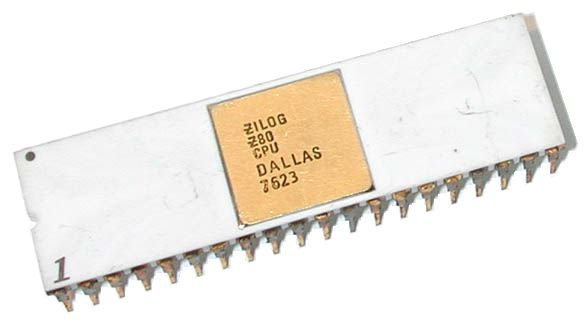
\includegraphics[width=0.25\textwidth]{z80}
\end{wrapfigure}

The Z80 CPU is a microprocessor invented by Zilog in 1975 as their first
product. It was designed as a largely software-compatible extension of the Intel
8080 CPU. Despite the Z80 being originally designed for use in embedded systems,
it gained massive popularity in the desktop market. The Z80 was used in
countless personal computers in the time period, such as the ZX 81, ZX Spectrum,
and Amstrad CPC. Many older game consoles also used this processor, notable the
Nintendo Gameboy and Sega Game Gear. In the modern day, the Zilog Z80 continues
to be used in Texas Instruments' line of TI-83/84 graphing calculators.

\section{Problem}

When programming for older computer systems, you have to take into account the
limited processing power and memory of these systems. Higher-level languages
have a performance overhead and their abstract nature prevents the programmer
from fully taking advantage of the available hardware. Even common "systems"
languages like C and C++ do not allow the programmer to have full control of
memory allocation, register usage, and what particular machine code instructions
are generated.

It is for this reason that retro computer programmers almost exclusively use an
assembly language for development. There is not just one clear-cut design for an
assembler, the level of complexity can vary greatly. For my end user's needs, we
deemed it adequate to use one of the more simple assembler designs: a 2-pass
assembler.

\subsection{Project requirements}

My end user likes to write games for old computer systems as a hobby, in
particular the Sinclair ZX Spectrum. When writing games for older systems, it is
vital that algorithms as optimised as possible. Taking advantage of quirks in
the processor are a must and these thing can only be done with an assembly
language.

When he is writing games in assembly, labels are frequently used to eliminate
the need to remember memory addresses when calling and jumping to subroutines
and other sections of the program. We decided that this feature would be
essential for the assembler to be useful.

The ability to use bases other than denary would also be essential as my end
user will frequently need to directly modify memory and manipulate data down to
the bits and bytes. This is made much easier when other bases such as binary and
hexidecimal can be used. For example, you may want to bitwise
\texttt{AND} a number by 15 to perform a modulo 16 operation. This is made far
clearer when written as 0x000F, as it is clearly shown that the lower nibble is
kept while the upper 24 bits are discarded. We decided that this feature would
also be essential if this assembler is to be useful.

One unique feature of the Z80 instruction set is its relative jump instructions.
These tell the CPU to add -128 to +127 to the program counter, depending on the
operand. My end user takes advantage of this instruction frequently, as the
instruction uses less memory (2 bytes instead of 3). So we agreed that designing
the assembler with support for relative jumps would be a neccesity.

When my end user is doing retro game development, he will often be using an
integrated development environment (IDE) such as Visual Studio Code to allow for
easy management of project files, version control, and syntax highlighting, to
name a few features. With this in mind, we agreed that the best way for a user
to interact with the assembler would be through command line options and
arguments. This allows for easy integration of the assembler into an IDE or
other custom build system, vastly speeding up development time.

%-------------------------------------------------------------------------------

\subsection{What is a 2-pass assembler?}

Unlike many programming languages, it is often the case than a program written
in assembly language will need to call/reference a label defined later on in the
program. If an assembler were to only read through the assembly source file
once, it would be impossible to resolve these forward label references. This is
because the assembler will have not yet encountered those label definitions, and
will therefore be unable to calculate the correct operand value in the outputted
machine code file.

To resolve this issue, an assembler can instead read through the source file
twice. During the first pass, all references to labels as operands can be
ignored. When a label definition is encountered, the assembler adds the
label name and its corresponding memory address to a symbol table.

During the second pass, if a label reference is encountered in an operand
argument, the symbol table is used to find the corresponding value. The value
can then be easily appended to the machine code file as the source file is being
read.

\subsection{Alternative assembler designs}

Apart from the 2-pass assembler, there are a few other common assembler designs.
A common design design found in most modern assemblers is the multiple-pass
design. These designs allow for the source code to be passed through as many
times as needed. This has the advantage of allowing support for symbol
definitions which rely on the values of other symbols later on in the code.
Although this assembler design is superior to a 2-pass assembler in execution,
the complexity of such an assembler is not far off that of a compiler. The added
complexity would increase development time too much while giving little benefit
to a retro computer programmer.

\subsection{The Z80 instruction set}

The main point of an assembler is to look up the opcode and operands contained
in a line and find the equivalent machine code instruction from the processor's
instruction set. The Z80 instruction set can be divided into 4 categories: main
instructins, extended instructions, ix/iy instructions, and bit instructions.

The main instructions are only 1 byte long and account for 90\% of the
instructions used in an assembly program.

The extended instructions are 2 bytes long and consist of many specialised
instructions which help for optimisations and are used less frequently.

The ix/iy instructions are all the instructions that use the Z80's index
registers. These are special purpose registers that usually point to the start
of a data structure, and can easily have offsets added to them to access members
of a particular structure. The instructions are also 2 bytes long.

The bit instructions are a vast amount of instructions that allow you to test
and set the individual bits of registers, memory addresses, index offsets, etc.
These instructions are also 2 bytes.

Here is a link to the entire Z80 instruction set: \url{https://clrhome.org/table/}

%-------------------------------------------------------------------------------

\section{System objectives}

\begin{enumerate}

\subsection{Required}

	\item \label{req_inputFile}
		Allow the input file to be specified on the command line
	\item \label{req_supportInstructions}
		Instruction set: support the main 256 Z80 instructions
	\item \label{req_doLabels}
		Support labels in the code
	\item \label{req_supportLiterals}
		Allow integer literals to be specified in denary and hexadecimal
	\item \label{req_calcOffset}
		Calculate the offset for relative jumps from a label
\subsection{Optional}

	\item Allow the output file to be specified
	\item Have an assembler directive that specifies the starting memory address
		(.org)
	\item Instruction set: support extended, ix/iy, and bit instructions
	\item Have assembler directives for placing arbitrary bytes into memory
		(.db, .dw)

\end{enumerate}



\chapter{Design}

\section{Getting command line arguments}

To begin this project, the first problem I decide to tackle is parsing command
line arguments. Once I get to the stage where a user can specify an input file
and possibly any options, that will set up a nice foundation on which the actual
assembler can be built.

To do this, I first test that the user has entered at least one command line
argument by testing the value of the \texttt{argc} variable, which is set
by the operating system when the program is run. This variables give the number
of command line arguments (including the name of the program itself), so I test
if the variable is 1 or less, and if so, print out some help text.

\begin{lstlisting}
// main.c
// line 30
if (argc <= 1) {
	usage(argv[0]);
	exit(EXIT_FAILURE);
}
\end{lstlisting}

The above referenced \texttt{usage()} function displays the help text, taking
the name of the called program as input.

\begin{lstlisting}
static void usage(char *argv0)
{
    fprintf(stderr, "usage: %s [-hv] [-o output_file] file\n", argv0);
}
\end{lstlisting}

In C, every command line argument is passed to \texttt{main()} as a member of an
array of strings: \texttt{argv}. So to access the first command line argument, I
would write \texttt{argv[1]}, as \texttt{argv[0]} would reference the program
name.

To parse the list of command line arguments, I use a \texttt{for} loop. The
loop iterates through every character in each member of \texttt{argv} and will
only proceed if the argument begins with a \texttt{'-'} character. As per the
usage string, every command line option must begin with a hyphen to indicate
that it is an option. Options can be combined into one argument or specified
seperately. For instance, \texttt{assembler -h -v} (to bring up the help menu
and display the version) could also be written as \texttt{assembler -hv}. When
an option is encountered, a \texttt{switch} statement executes the correct
branch of code to satisfy that option.

The very last argument will always be interpreted as the input file name, and
an error will be thrown if this file name is not provided.

The options I implement are help (\texttt{-h}), version (\texttt{-v}), and
output file (\texttt{-o [filename]}). The output file name is copied into the
variable \texttt{outfile\_name} which is initialised to \texttt{"out.bin"} if
this option is not used.

\begin{lstlisting}
	char outfile_name[64] = "out.bin";

	int o = 1; // the char index into the argument string
    int i;
    for (i = 1; *(argv[i]) == '-' && i < argc; o++) {
        switch (argv[i][o]){
        case 0:     // go to next argument
            o = 0;
            i++;
            break;
        case 'h':
            usage(argv[0]);
            exit(EXIT_SUCCESS);
        case 'v':
            version();
			exit(EXIT_SUCCESS);
		case 'o':
			if (argc < i + 3) die("No output filename provided");
			i++;
			strncpy(outfile_name, argv[i], 63);
			if (strlen(outfile_name) != strlen(argv[i])) {
				die("Output filename too long");
			}
			o = 0;
			i++;
			break;
        default:
			usage(argv[0]);
			exit(EXIT_FAILURE);
        }
        if (i == argc) die("No input filename provided");

    }

	if (argc > i + 1) die("Multiple files specified");
\end{lstlisting}

\section{Pass 1: symbol table}

Now that the input file and output file names have been retrieved, I can proceed
to implement the first pass of the assembler: the symbol table.

Because the number of symbols defined in a source file is unknown, I decide to
use a linked list to store the symbol table entries. Linked lists allow for the
size of the list to change dynamically, and no memory will be wasted if the
list ends up being smaller than the allocated size. If I weren't to use a linked
list, I would either have to do another pass to find the number of labels, or I
would have to allocate a list of an arbitrarily large size. The former
alternative isn't ideal as an extra pass would cause the program to no longer be
a `2-pass assembler'. The latter alternative is unsuitable because if the user
defines too many symbols, the assembler will be unable to assemble the code.

I define each element of the linked list as a structure that holds the symbol
name, symbol value, and a pointer to the next element in the list. I then declare
the functions used to access and modify the symbol table.

\begin{lstlisting}
struct symbol {
	const char *label;
	int value;
	struct symbol *next;
};

size_t symtable_len(const struct symbol *symtable_head);
int symtable_search(const struct symbol *symtable_head, const char *label);
size_t symtable_build(FILE *fp, struct symbol **symtable_head);
void symtable_print(struct symbol *symtable_head);
\end{lstlisting}

\texttt{symtable\_len()} is a simple function that loops through every symbol
entry's \texttt{next} pointer until it encounters the end of the list. The
number of iterations is the returned length of the list.

\texttt{symtable\_search()} perfoms a linear search on the list, returning the
value which corresponds to the specified label name;

\bigbreak

Of the four functions just declared, \texttt{symtable\_build()} is the most
important, as it is the function that does the entire first pass of the
assembler.

This function works by looping through every line of the source file, important
information from the line, such as if any labels are defined, as well as any
opcode or operands are retrieved via the \texttt{parseline()} function. This
function returns its data in a structure which is layed out as follows:

\begin{lstlisting}
struct line_data {
	
	char *new_label; // empty if no label is defined

	ssize_t opcode_sz; // if 0, no opcode
	uint8_t opcode[3]; // start at [0]
	enum OpcodesPseudo pseudo_op; // use if opcode_sz == -1

	size_t operand_sz; // if 0, no operand
	char operand_label[LABEL_MAX_LEN+1]; // when empty, use operand_literal instead
	uint16_t operand_literal; // little endian
};
\end{lstlisting}

This function is not yet implemented at this stage, but it can be treated as a
black box which returns all vital information from the current line.

For the first pass, the only returned piece of information that's important is
the \texttt{new\_label} member, which, if not equal to \texttt{NULL} will
contain the name of a newly defined label.

If a new label is defined, I add the symbol to the linked list by allocating
memory for a new entry using \texttt{calloc()} and set the entry's \texttt{next}
pointer to the current head of the linked list. I then make this entry the
head of the linked list.

\begin{lstlisting}
	if (data.new_label != NULL) {
		struct symbol *new_symbol = calloc(sizeof(struct symbol), 1);
		new_symbol->label = data.new_label;
		new_symbol->value = address;
		new_symbol->next = *symtable_head;
		*symtable_head = new_symbol;
	}
\end{lstlisting}

Since the purpose of the first pass is to build a list of symbol names which are
mapped to memory addresses, the first pass will have to check if a line contains
the \texttt{.org} pseudo-instruction. This instruction changes the current
memory address of assembled code proceeding it. Therefore, any label definitions
after a \texttt{.org} pseudo-instruction will have to take this into account.

After checking if the current line contains a label definition, I check if the
current line contains a \texttt{.org} call. If it does, I change the current
assembly address to the argument of \texttt{.org}. To support
pseudo-instructions, I test for a special case where the opcode size is
\texttt{-1}. This indicates that the current opcode is in fact a pseudo-opcode.

\begin{lstlisting}
if (data.opcode_sz == -1 && data.pseudo_op == PSEUDO_ORG) {
	if (data.new_label != NULL) die("Cannot define label on same line as .ORG");
	if (data.operand_label[0] != '\0') {
		die("ERROR on line %d: .ORG cannot use labels\n", line_no);
	}
	address = data.operand_literal;
}
\end{lstlisting}

At the end of every iteration, I increment the current assembly address by the
size of the current instrution in bytes.

\begin{lstlisting}
address += line_assembled_size;
\end{lstlisting}

\section{Pass 2: assembly}

Now that the symbol table has been built, it is possible to pass through the
file only once more. I wrap this entire second pass in the \texttt{assemble()}
function, which takes the currently open file, the symbol table, and the output
memory buffer as arguments.

\begin{lstlisting}
void assemble(FILE *fp, const struct symbol *symtable_head, char *memory);
\end{lstlisting}

Just like the \texttt{symtable\_build()} function used to perform the first
pass, a \texttt{while} loop is used to pass through the file, and the
\texttt{parseline()} function is used to get important data from the line.

After retrieving the opcode, operands, and any label definitions on the line
(all returned from \texttt{parseline()}), I first test if the opcode size is
greater than \texttt{0}, as \texttt{0} means that there is no instruction on the
line, and \texttt{-1} means that the instruction on the line is a
pseudo-instruction.

Every byte of the opcode is then copied into the output buffer, proceeded by the
operand. However, if the current operand is a label reference, the symbol table
is checked to retrieve the correct value in place of this label name.

\begin{lstlisting}
if (data.opcode_sz > 0) {
	// copy opcode
	for (unsigned int i = 0; i < data.opcode_sz; i++) {
		memory[memindex++] = data.opcode[i];
	}

	// get operand
	uint16_t operand;
	if (data.operand_label[0] != '\0') {
		int symbol_value = symtable_search(symtable_head, data.operand_label);
		if (symbol_value == -1) {
			die("undefined label %s on line %d\n", data.operand_label, line_no);
		}
		operand = (unsigned)symbol_value & 0xFFFF;
	} else {
		operand = data.operand_literal;
	}

	// copy operand
	for (unsigned int i = 0; i < data.operand_sz; i++) {
		memory[memindex++] = (operand >> (i * 8)) & 0xFF;
	}
\end{lstlisting}

Just like in the first pass, I again test for the \texttt{.org}
pseudo-instruction and modify the current memory address accordingly. The reason
that I need to keep track of the current assembly address in the second pass is
because the Z80 has a few relative jump instructions. These instructions take as
an operand a twos-complement integer which represents the value which must be
added to the program counter to reach the referenced label. This is implemented
by simply subtracting the label address from the current address.

\begin{lstlisting}
// compute offset if instruction is relative jump
if (	data.opcode_sz == 1			&&
	   (data.opcode[0] == JR_N		||
		data.opcode[0] == JR_NZ_N	||
		data.opcode[0] == JR_Z_N	||
		data.opcode[0] == JR_NC_N	||
		data.opcode[0] == JR_C_N	||
		data.opcode[0] == DJNZ_N)	) {
	signed int offset = (signed int)operand - (signed int)address - 2;
	if (offset > 127 || offset < -128) {
		die("relative jump too far");
	}
	operand = (int8_t)offset;
}
\end{lstlisting}

Just as in the first pass, the current address is again incremented by the size
of the parsed instruction.

This is the end of the second pass.

\begin{lstlisting}
address += line_assembled_size;
\end{lstlisting}

Back in \texttt{main()}, the new \texttt{assemble()} function is called after
allocating space for the output file and rewinding the file pointer so that it
points to the beginning of the source file.

\begin{lstlisting}
// SECOND PASS
char* memory = calloc(memory_size, 1);
if (memory == NULL) die("Failed calloc()");
rewind(fp);
assemble(fp, symtable_head, memory);
fclose(fp);
\end{lstlisting}

\section{Parsing and decoding a line of assembly}

Now that the foundations of the assembler have been constructed, the main part
of the program that is missing is the \texttt{parseline()} function. Which until
now, has been left as a black box which does the neccesary processing to return
useful information from any given line of Z80 assembly.

There are 3 seperate pieces of data that must be retrieved from a line of
assembly. These are: the opcode (in machine code), the operand (whether a
literal or a label reference), and the name of the label defined on that line.
All of these fields are optional. A line may only contain an opcode and a line
may only contain a label definition, for instance. The only exception to this
rule is that a line must contain an opcode if there is also an operand.

To start off with, the first column of the line is checked to see if it is the
start of a comment (indicated by the semicolon character). If this is the case,
the function can safely return, having not found any instruction or label
definition.

\begin{lstlisting}
data->new_label = NULL;
data->opcode_sz = 0;
data->operand_sz = 0;
data->operand_label[0] = '\0';

if (line[0] == ';') return 0;
\end{lstlisting}

\subsection{Label definitions}

As a rule of my assembly language syntax, all label definitions must begin from
the first column of the line. They can only contain alphanumeric characters and
underscores but the first character cannot be numeric.

I check for this by looping through character-by-character, testing for many
conditions in the process. First, if the character is a semicolon, if it is,
the loop will exit as this is a comment. Second, I check if the current
character would be a valid label character. If it is, the current character will
be appended to the label name. If it is not, I check that the character is
either a tab, space, new line, or colon. As these are the only characters which
can appear after a label definition. If any of these characters are encountered,
the loop is ended.

\begin{lstlisting}
int len = 0;
for ( ;; ) { // infinite loop
	if (line[len] == ';')  break;
	int char_type = is_label_char_valid(line[len]);
	if (char_type == 1) len++;
	if (char_type == 0) {
		if (	line[len] != '\t' &&
				line[len] != '\n' &&
				line[len] != ' ' &&
				line[len] != ':') {
			die("line %d: Label contains an invalid character\n", line_no);
		} else {
			break;
		}
	}
}
\end{lstlisting}

The label is copied over and converted to lowercase as this assembler is not
case-sensitive. \texttt{malloc()} is used to allocate memory for this label

\begin{lstlisting}
data->new_label = malloc(len + 1);
for (int i = 0; i < len; i++) {
	data->new_label[i] = tolower(line[i]);
}
data->new_label[len] = '\0'; // add terminating 0
\end{lstlisting}

If a colon was specified after the label, it is then skipped over:

\begin{lstlisting}
if (line[index] == ':') {
	index++;
}
\end{lstlisting}

\subsection{Getting the opcode}

After a label definition, there must be tabs or spaces seperating it from the
opcode. I skip over them with a \texttt{for} loop.

\begin{lstlisting}
for ( ; line[index] == '\t' || line[index] == ' '; index++) ;
\end{lstlisting}

The opcode is copied over in a similar way to the label definition. The line
is looped through from the end of the label definition until a tab, space,
new line, or comment is encountered. Every character is checked to see if it
would be valid in an opcode using the \texttt{opcode\_char\_valid()} function.

The index variable is the same one used previously, so its current position will
be after the label definition and any whitespace following it.

\begin{lstlisting}
int len = 0; // length of opcode name
char opcode_name[OPCODE_NAME_MAX_LEN + 1] = { 0 };
for ( ;; ) { // infinite loop
	if (line[index] == ';') break;
	int char_valid = is_opcode_char_valid(line[index]);
	if (char_valid == 1) {
		// char is valid
		opcode_name[len] = line[index];
		len++;
		index++;
		if (len > OPCODE_NAME_MAX_LEN) {
			die("line %d: Opcode name too long\n", line_no);
		}
	} else {
		// char is not valid or is end of opcode
		if (	line[index] != '\n' &&
			line[index] != '\t' &&
			line[index] != ' '	) {
			die("line %d: Opcode contains invalid characters, char: %c\n", line_no, line[index]);
			exit(EXIT_FAILURE);
		} else break;
	}
}
if (strlen(opcode_name) == 0) return 0;
\end{lstlisting}

The \texttt{is\_opcode\_char\_valid()} function just checks each character and
only allows letters or a full-stop (for pseudo instructions).

\begin{lstlisting}
if (isalpha(c)) return true;
if (c == '.') return true;
else return false;
\end{lstlisting}

The name of the opcode is now stored in the \texttt{opcode\_name} variable.

\subsection{Getting the operands}

In my assembler's syntax, operands are specified as either numbers, labels, or
a register, any of which may also be surrounded by brackets. For example,
\texttt{(hl)}, \texttt{0x33}, and \texttt{myLabel} would be valid operands.

If there are multiple operands, they will all be saved into the same string at
this stage, their actual values will be parsed later.

To copy the operands string, I loop through the rest of the line until
encountering either a new line or a comment. Similar to what I did with the
opcode, I use the \texttt{is\_operand\_char\_valid()} function to avoid parsing
any invalid characters later on.

\begin{lstlisting}
int operand_str_size = 0;
char *start_of_operand = line + index;
for ( ;; ) {
	if (line[index] == ';') break;
	int char_valid = is_operand_char_valid(line[index]);
	if (char_valid == 1) {
		operand_str_size++;
		index++;
	}
	if (char_valid == 0) {
		if (line[index] != '\n') {
			die("ERROR: line %d: operand contains invalid character: %2X (hex)\n", line_no, line[index]);
		} else break;
	}
}
char *operand_str = NULL;
if (operand_str_size != 0) {
	operand_str = malloc(operand_str_size + 1);
	memcpy(operand_str, start_of_operand, operand_str_size);
	operand_str[operand_str_size] = 0; // null terminator
}
\end{lstlisting}

The \texttt{is\_operand\_char\_valid()} function serves as a simple filter that
rejects operands that are definitely invalid:

\begin{lstlisting}
if (isalnum(c)) return true;
switch (c) {
case ' ':
case '+':
case '-':
case '_':
case '(':
case ')':
case ',':
case '\'':
case '\t':
		return true;
default:
		return false;
}
\end{lstlisting}

\subsection{Parsing the instruction}

Now that the opcode and operand strings have been retrieved, they are passed
into the \texttt{instruction\_lookup()} function which stores the operand's
machine code value and converted operands into a custom data structure.

\begin{lstlisting}
// figure out what the instruction is
instruction_lookup(opcode_name, operand_str, data);
\end{lstlisting}

The now-modified \texttt{data} variable is returned by the \texttt{parseline()}
function. This variable now contains the name of any newly defined label, the
correct binary opcode, and any converted operands.

\texttt{instruction\_lookup()} takes three arguments; the first two are the
operand and opcode strings respectively; the final argument is the previously
mentioned \texttt{data} variable which is passed by-reference so that it can be
modified by the function.

\subsubsection{Parsing pseudo-opcodes}

Firstly, the opcode name is checked to see if it begins with a full-stop. If it
does, the opcode is checked against the assembler's pseudo-opcodes, of which
there is only one, \texttt{.org}. If the opcode is \texttt{.org}, the operand
string is converted to an integer using the function \texttt{strtol()}, which
converts either a denary or hexadecimal number into an integer. Strings starting
with \texttt{"0x"} are treated as hexadecimal.

The function then returns, storing the operand value as the specified memory
address.

\begin{lstlisting}
static void instruction_lookup(const char *opcode_name, char *operand_name, struct line_data *data) {
	switch (opcode_name[0]) {
		case '.':
			if (strcmp(opcode_name + 1, "org") == 0) {

				uint16_t newAddr;
				newAddr = (uint16_t)strtol(operand_name, NULL, 0);

				// -1 means pseudo opcode
				data->opcode_sz = -1;
				data->pseudo_op = PSEUDO_ORG;
				data->operand_sz = 2;
				data->operand_label[0] = '\0';
				data->operand_literal = newAddr;
			}
			break;
\end{lstlisting}

\subsubsection{Parsing regular instructions}

If the opcode does not begin with a full-stop, it is treated as a real opcode.
The opcode and operand strings are then passed into another function,
\texttt{instruction\_parse()}.

\begin{lstlisting}
		default:
			{	// NORMAL INSTRUCTION
				struct ParsedInstruction instruction;
				instruction = instruction_parse(opcode_name, operand_name);
\end{lstlisting}

This function does two things: it converts the opcode string to lowercase, and
splits up the operand string into many parts. These parts can be seen in the
sub-structure of \texttt{ParsedInstruction}, \texttt{ParsedOperand}:

\begin{lstlisting}
struct ParsedOperand {
	bool isIndirect;			// does the operand use (  ) ?
	char reg[LABEL_MAX_LEN+1];	// can also be a flag or label
	signed int value;
};
\end{lstlisting}

\texttt{isIndirect} is a boolean member that is true if the operand uses
indirect addressing.

\texttt{reg} is a string that holds whatever text is contained in the operand,
if any. Despite the name, it does not neccesarily have to hold the name of a
register, and could be a label or a flag.

\texttt{value} is set equal to whatever numeric value is contained in the
operand. This value is ignored unless \texttt{reg} is an empty string.

Here is an example of how this data structure would hold the operands of the
instruction \texttt{ld (hl), 0xFF}:

\begin{lstlisting}
operand1.isIndirect = true;
operand1.reg = "hl";
// operand1.value is ignored

operand2.isIndirect = false;
operand2.reg = NULL; // (empty)
operand2.value = 255;
\end{lstlisting}

To do this parsing, the operands must first be split up into composite strings.
A \texttt{for} loop iterates through the string until it finds a comma.

\begin{lstlisting}
for (int i = 0; args[i] != '\0'; i++) {

	// convert tabs to spaces
	if (args[i] == '\t') args[i] = ' ';

	// find if there is a comma, and replace with '\0' to split operands
	if (args[i] == ',') {
		args[i] = '\0';
		arg2 = args + i + 1;
	}
}
\end{lstlisting}

From this point, the two operands are seperately passed into the function
\texttt{operand\_parse()}, which parses the operand into the aforementioned
\texttt{ParsedOperand} data structure.

\subsubsection{Parsing the operands}

Firstly, the string is searched for a left-bracket and right-bracket character.

\begin{lstlisting}
const char* lbkt_loc = strchr(arg, '(');
const char* rbkt_loc = strchr(arg, ')');
\end{lstlisting}

If both brackets are present (and the left bracket comes first), the
\texttt{isIndirect} boolean variable is set to true.

\begin{lstlisting}
if (lbkt_loc != NULL && rbkt_loc != NULL) {
	po.isIndirect = true;
	if (lbkt_loc > rbkt_loc) {
		die("mismatched brackets with operand: %s", arg);
	}
} else {
	po.isIndirect = false;
}
\end{lstlisting}

The operand string is then looped through until an alphabetical character is
encountered. From then on, every subsequent letter is added to the \texttt{reg}
variable.

The remainder of the operand is then stepped through to see if any numerical
characters are encountered. And if so, they are combined and converted into an
integer, to be stored in \texttt{value}. The string is also checked for
\texttt{0x}, as this specifies that the integer is hexadecimal.

\begin{lstlisting}
if (num_start != NULL) {
	// copy it into buffer
	char num_buffer[16] = { 0 };
	for (int i = 0; i < 15; i++) {
		if ( isdigit(num_start[i]) || ('a' <= tolower(num_start[i]) && tolower(num_start[i]) <= 'f') || ( ( i == 1 || i == 2 ) && tolower(num_start[i]) == 'x') ||
				( i == 0 && ( (num_start[i] == '+') || (num_start[i] == '-') ) )
				  ) { // 'x' is in case of hexadecimal
			num_buffer[i] = num_start[i];
		} else {
			num_buffer[i] = '\0';
			break;
		}
	}

	// convert it to integer
	int num = strtol(num_buffer, NULL, 0); // 0 base means either 10, 8, or 16 depending on input
	po.value = (signed int)num;
}
\end{lstlisting}

\subsection{Decoding the parsed instruction}

Now that the instruction has been split up into its composite parts, the parsed
information is passed into the \texttt{instruction\_decode()} function. This
function finds the correct machine-code instruction by looking at the opcode
name and the format of the operands.

The Z80 CPU has 256 main machine-code instructions which only take up 1 byte per
opcode. To decode these, I make a 256-long list which maps opcode names and
operand formats to their equivelent instructions.

Each entry in the list has this format:

\begin{lstlisting}

struct InstructionDecodeEntry {
	// opcode is the entry's index in the list

	// result
	size_t	operand_sz;

	// pattern to match
	const char 	   *p_instruction_name;
	int				p_operand_count;
	// operand 1
	bool			p_op1_indirect;
	const char		p_op1_reg[LABEL_MAX_LEN+1];
	// operand 2
	bool			p_op2_indirect;
	const char		p_op2_reg[LABEL_MAX_LEN+1];
};

\end{lstlisting}

The \texttt{operand\_size} member is the size in bytes that the data immediately
following the opcode will take up in memory. This data is usually a value
specified as an operand.

The \texttt{p\_instruction\_name} is the name of the parsed instruction, which
will be the same as the opcode in the assembly source file. For example:
\texttt{ld}, \texttt{ldir}, or \texttt{out}.

The \texttt{p\_opx\_indirect} members specify whether or not the instruction
operands use indirect addressing.

The \texttt{p\_opx\_reg} members specify the register or flag name that must
appear in that operand for the instruction to match.

For many instruction, there are fewer than two operands. In these cases,
\texttt{p\_op2\_reg} and/or \texttt{p\_op1\_reg} may be left empty to indicate
that the operand should be left empty for the instruction to match.

Below are the first few entries in the decode table, to demonstrate how
instructions are matched.

\begin{lstlisting}
const struct InstructionDecodeEntry DECODE_TABLE_MAIN[] = {
	// 0x00
	{	0,	"nop",	0,								}, // nop
	{	2,	"ld",	2,	false,	"bc",	false,	""	}, // ld bc, **
	{	0,	"ld",	2,	true,	"bc",	false,	"a"	}, // ld (bc), a
	{	0,	"inc",	1,	false,	"bc",				}, // inc bc
	{	0,	"inc",	1,	false,	"b",				}, // inc b
	{	0,	"dec",	1,	false,	"b",				}, // dec b
	{	1,	"ld",	2,	false,	"b",	false,	""	}, // ld b, *
	{	0,	"rlca",	0,								}, // rlca
	// etc...
};
\end{lstlisting}

To find the correct instruction, the function begins by looping through the
entire list. Once an entry is found to match the parsed opcode and operands,
the current value of the  \texttt{i} variable is the correct machine op-code.

\begin{lstlisting}
for (int i = 0; i < (int)(sizeof(DECODE_TABLE_MAIN) / sizeof(struct InstructionDecodeEntry)); i++) {
\end{lstlisting}

\subsubsection{Checking for a match}

Firstly, the opcode name passed as an argument is compared to the opcode name of
the current entry in the list. If this is the case, further conditions are
checked.

\begin{lstlisting}
if (strcmp(e.p_instruction_name, p.opcode) == 0) {
\end{lstlisting}

\subsubsection{If there are no operands}

If there are no operands, then you can be 100\% certain that this is a match.

\begin{lstlisting}
if (e.p_operand_count == 0) {
	d.opcode_sz = 1;
	d.opcode[0] = i;
	d.operand_sz = 0;
	d.operand_label[0] = 0;
	break;
}
\end{lstlisting}

\subsubsection{If there are one or more operands}

If there are one or more operands, the comparison becomes complicated.

First of all, the \texttt{isIndirect} flags are compared to ensure that if the
instruction requires brackets, that these brackets are present. If the
\texttt{isIndirect} flags do not match, \texttt{continue} is used to skip over
this iteration and check the next entry in the table.

\begin{lstlisting}
if (e.p_operand_count >= 1) {
	if (e.p_op1_indirect != p.operand1.isIndirect) continue;
	if (e.p_operand_count == 2 && (e.p_op2_indirect != p.operand2.isIndirect) ) continue;
\end{lstlisting}

\subsubsection{If there is only one operand}

If there is only one operand, then there are two possible outcomes. The first
outcome is that the current entry's operand does not specify a string. In that
case, the operand's value (or label, if present) will be inserted immediately
after the opcode in memory.

\begin{lstlisting}
// example: jp 23456
if (e.p_op1_reg[0] == 0) {
	// op1 value is definitely operand
	if (p.operand1.reg[0] == 0) { // if no label, use value
		d.operand_label[0] = 0;
		d.operand_literal = p.operand1.value;
	} else { // copy over the label name, this will be replaced in pass 2
		strncpy(d.operand_label, p.operand1.reg, LABEL_MAX_LEN+1);
	}
	d.opcode_sz = 1;
	d.opcode[0] = i;
	d.operand_sz = e.operand_sz;
	break;
}
\end{lstlisting}

The second outcome is that the current entry's operand specifies a string. In
that case, the operand string must exactly match the current entry's operand. No
data will be copied after the instruction.

\begin{lstlisting}
else if (strcmp(e.p_op1_reg, p.operand1.reg) == 0) { // check if exact match
	d.opcode_sz = 1;
	d.opcode[0] = i;
	d.operand_sz = 0;
	d.operand_label[0] = 0;
	break;
}
\end{lstlisting}

If neither of these conditions are met, \texttt{continue} is used to skip over
this iteration and check the next entry in the table.

\begin{lstlisting}
else continue;
\end{lstlisting}

\subsubsection{If there are two operands}

If there are two operands, there are three possible conditions that are valid.

The first condition is that the first operand's string matches and the second
operand's string matches. In this case, there is no extra data to be added after
the machine instruction in memory.

\begin{lstlisting}
if ( e.p_op1_reg[0] != 0 && e.p_op2_reg[0] != 0 ) {
	if (strcmp(e.p_op1_reg, p.operand1.reg) != 0) { // compare first operand
		continue;
	}
	if (strcmp(e.p_op2_reg, p.operand2.reg) != 0) { // compare second operand
		continue;
	}
	// MATCH,	MATCH
	d.opcode_sz = 1;
	d.opcode[0] = i;
	d.operand_sz = 0; // there is no extra data
	d.operand_label[0] = 0;
	break;
}
\end{lstlisting}

The second condition to check is that the entry's first operand is empty, which
means there is a value or label to copy. And also that the entry's second
operand contains a string which exactly matches the operand in the source file.

In this case, the value or label (if present) will be inserted immediately after
the machine op-code in memory.

\begin{lstlisting}
else if (	e.p_op2_reg[0] != 0 && // second operand is a value/label
			strcmp(e.p_op2_reg, p.operand2.reg) == 0 && // first operand matches
			e.operand_sz != 0	) { // the instruction actually needs subsequent data
	// LBL_VAL,		MATCH
	if (p.operand1.reg[0] == 0) {
		d.operand_label[0] = 0;
		d.operand_literal = p.operand1.value;
	} else { // if there is a label, copy it. It will be replaced on the second pass.
		if (label_is_reserved(p.operand1.reg)) continue;
		strncpy(d.operand_label, p.operand1.reg, LABEL_MAX_LEN+1);
	}
	d.opcode_sz = 1;
	d.opcode[0] = i;
	d.operand_sz = e.operand_sz;
	break;
}
\end{lstlisting}

The third condition to check is that the entry's first operand contains a string
which exactly matches the operand in the source file. And also that the entry's
second operand is empty, which means there is a value or label to copy.

This is exactly the same as the second condition, except that the operands are
the other way round.

If none of these conditions are met, the loop with simply continue and check the
remaining entries in the list.

If the loop finishes before finding a matching instruction, an error will be
displayed telling the user that the instruction cannot be found.

\begin{lstlisting}
if (d.opcode_sz == 0) {
	die("unknown instruction");
}
\end{lstlisting}

\subsubsection{Other instructions}

Although the main 256 assembly instructions can now be assembled, there are
still many instructions remaining. The process of decoding these extended
instructions is pretty much the same, and many can be added manually.

I add some of the most commonly used extended instructions similarly to before,
except that these instructions are checked manually instead of using a table.

\begin{lstlisting}
// one example, "sra b"
if (	(strcmp(p.opcode, "sra") == 0) &&
		p.operands == 1 &&
		p.operand1.isIndirect == false &&
		(strcmp(p.operand1.reg, "b") == 0)){
			d.opcode_sz = 2;
			d.opcode[0] = 0xCB;
			d.opcode[1] = 0x28; // extended instructions are multi-byte
			d.operand_sz = 0;
			d.operand_label[0] = 0;
}
\end{lstlisting}

%-------------------------------------------------------------------------------

\chapter{Technical Solution}

\section{Source files}

\lstset{numbers=left}

\subsection{main.c}
\lstinputlisting{../src/main.c}
\subsection{symtable.c}
\lstinputlisting{../src/symtable.c}
\subsection{assemble.c}
\lstinputlisting{../src/assemble.c}
\subsection{parseline.c}
\lstinputlisting{../src/parseline.c}
\subsection{util.c}
\lstinputlisting{../src/util.c}

\section{Header files}

\subsection{symtable.h}
\lstinputlisting{../src/symtable.h}
\subsection{assemble.h}
\lstinputlisting{../src/assemble.h}
\subsection{parseline.h}
\lstinputlisting{../src/parseline.h}
\subsection{util.h}
\lstinputlisting{../src/util.h}



\chapter{Testing}

\section{Testing for required objective \ref{req_inputFile}}

\subsubsection{Allow the input file to be specified on the command line}

\subsection{Testing table}

\begin{table}[H]
	\resizebox{\textwidth}{!}{%
\begin{tabular}{@{}llllllll@{}}
\toprule
No. & Test Description                         & Data Type & Input                         & Expected Result                 & Actual Result                                         & Pass? & Improvement needed? \\ \midrule
1   & Specify an input file that exists        & String    & assembler file.asm            & File is opened                  & Successfully assembled, file was opened                                        & Y     & No                  \\
2   & Specify an input file that doesn't exist & String    & assembler notreal.asm         & Descriptive error message given & ERROR: No such file or directory                      & Y     & Show a help message                  \\
3   & Specify a directory as an input file     & String    & assembler src/                & Descriptive error message given & ERROR: A regular file must be specified               & Y     & Show a help message                  \\
4   & Do not give a file name                  & String    & assembler                     & Help message shown              & usage: assembler {[}-hv{]} {[}-o output\_file{]} file & Y     & No                  \\
5   & Specify multiple input files             & String    & assembler test1.asm test2.asm & Descriptive error message given & ERROR: Multiple files specified                       & Y     & Show a help message                  \\ \bottomrule
\end{tabular}}
\end{table}

\subsection{Evidence}

\lstset{numbers=none}
\lstset{language=sh}
\begin{lstlisting}
$ assembler file.asm
$ ls out.bin
out.bin
$ assembler notreal.asm
ERROR: No such file or directory
$ assembler ../src/
ERROR: A regular file must be specified
$ assembler
usage: assembler [-hv] [-o output_file] file
$ assembler file.asm test.asm
ERROR: Multiple files specified
\end{lstlisting}





\section{Testing for required objective \ref{req_supportInstructions}}

\subsubsection{Instruction set: support the main 256 Z80 instructions}

\subsection{Testing table}

\begin{table}[H]
	\resizebox{\textwidth}{!}{%
\begin{tabular}{@{}llllllll@{}}
\toprule
No. & Test Description                                 & Data Type     & Input       & Expected Result                                                                                                 & Actual Result              & Pass? & Improvement needed?       \\ \midrule
1   & Assemble a single valid instruction              & Assembly file & ld hl, 123  & 21 7B 00                                                                                                        & 21 7B 00                   & Y     & No                        \\
2   & Try assemble an instruction with invalid operand & Assembly file & ld xy, 123  & Error, unknown instruction                                                                                      & ERROR: Unknown instruction & Y     & Show line number of error \\
3   & Try assemble an instruction with invalid opcode  & Assembly file & mov a, 123  & Error, unknown instruction                                                                                      & ERROR: Unknown instruction & Y     & Show line number of error \\
4   & Assemble all main 256 instructions               & Assembly file & (see below) & \begin{tabular}[c]{@{}l@{}}A clear pattern of ascending numbers\\ as the instructions are in order\end{tabular} & (see below)                & Y     & No                       \\
	5   & Assemble a division routine               & Assembly file & (see below) & (see below) & (see below)                & Y     & No                       \\ \bottomrule
\end{tabular}}
\end{table}

\subsection{Evidence}

\begin{lstlisting}
sh-5.1$ cat 1.asm
	ld hl, 123
sh-5.1$ assembler -o 1.bin 1.asm
sh-5.1$ hexdump -C 1.bin
00000000  21 7b 00                                          |!{.|
00000003


sh-5.1$ cat 2.asm
	ld xy, 123
sh-5.1$ assembler -o 2.bin 2.asm
ERROR: unknown instruction



sh-5.1$ cat 3.asm
	mov a, 123
sh-5.1$ assembler -o 3.bin 3.asm
ERROR: unknown instruction



sh-5.1$ cat 4.asm
	.org	0
	nop
	ld		bc, 0
	ld		(bc), a
	inc		bc
	inc		b
	dec		b
	ld		b, 0
	rlca
	ex		af, af'
	add		hl, bc
	ld		a, (bc)
	dec		bc
	inc		c
	dec		c
	ld		c, 0
	rrca

	djnz	0
	ld		de,	0
	ld		(de), a
	inc		de
	inc		d
	dec		d
	ld		d, 0
	rla
	jr		0
	add		hl, de
	ld		a, (de)
	dec		de
	inc		e
	dec		e
	ld		e, 0
	rra
	
	jr		nz, 0
	ld		hl,	0
	ld		(0), hl
	inc		hl
	inc		h
	dec		h
	ld		h, 0
	daa
	jr		z, 0
	add		hl,hl
	ld		hl, (0)
	dec		hl
	inc		l
	dec		l
	ld		l, 0
	cpl

	jr		nc, 0
	ld		sp, 0
	ld		(0), a
	inc		sp
	inc		(hl)
	dec		(hl)
	ld		(hl), 0
	scf
	jr		c, 0
	add		hl, sp
	ld		a, (0)
	dec		sp
	inc		a
	dec		a
	ld		a, 0
	ccf

	ld		b, b
	ld		b, c
	ld		b, d
	ld		b, e
	ld		b, h
	ld		b, l
	ld		b, (hl)
	ld		b, a
	ld		c, b
	ld		c, c
	ld		c, d
	ld		c, e
	ld		c, h
	ld		c, l
	ld		c, (hl)
	ld		c, a

	ld		d, b
	ld		d, c
	ld		d, d
	ld		d, e
	ld		d, h
	ld		d, l
	ld		d, (hl)
	ld		d, a
	ld		e, b
	ld		e, c
	ld		e, d
	ld		e, e
	ld		e, h
	ld		e, l
	ld		e, (hl)
	ld		e, a

	ld		h, b
	ld		h, c
	ld		h, d
	ld		h, e
	ld		h, h
	ld		h, l
	ld		h, (hl)
	ld		h, a
	ld		l, b
	ld		l, c
	ld		l, d
	ld		l, e
	ld		l, h
	ld		l, l
	ld		l, (hl)
	ld		l, a
sh-5.1$ assembler -o 4.bin 4.asm
sh-5.1$ hexdump -C 4.bin
00000000  00 01 00 00 02 03 04 05  06 00 07 08 09 0a 0b 0c  |................|
00000010  0d 0e 00 0f 10 ea 11 00  00 12 13 14 15 16 00 17  |................|
00000020  18 de 19 1a 1b 1c 1d 1e  00 1f 20 d4 21 00 00 22  |.......... .!.."|
00000030  00 00 23 24 25 26 00 27  28 c6 29 2a 00 00 2b 2c  |..#$%&.'(.)*..+,|
00000040  2d 2e 00 2f 30 ba 31 00  00 32 00 00 33 34 35 36  |-../0.1..2..3456|
00000050  00 37 38 ac 39 3a 00 00  3b 3c 3d 3e 00 3f 40 41  |.78.9:..;<=>.?@A|
00000060  42 43 44 45 46 47 48 49  4a 4b 4c 4d 4e 4f 50 51  |BCDEFGHIJKLMNOPQ|
00000070  52 53 54 55 56 57 58 59  5a 5b 5c 5d 5e 5f 60 61  |RSTUVWXYZ[\]^_`a|
00000080  62 63 64 65 66 67 68 69  6a 6b 6c 6d 6e 6f        |bcdefghijklmno|
0000008e



sh-5.1$ cat 5.asm
; math.z80

; div_d_e
; performs integer division d / e
; d - quotient, a - remainder
div_d_e
	xor	a
	ld	b, 8
div_d_e_loop
	rla
	cp	e
	jr	div_d_e_2
	sub	e
	inc	d
div_d_e_2
	djnz	div_d_e_loop
	ret

; quotient goes in ac
; remainder goes in hl
div_ac_de:
	ld	hl, 0
	ld	b, 16
div_ac_de_loop:
	rla
	jr	div_ac_de_2
	add	hl, de
	dec	c
div_ac_de_2
	djnz	div_ac_de_loop
	ret

;### CMPGTE -> test if A>=B
;### Input      HL=A, DE=B
;### Output     HL=1, CF=0 -> true
;###            HL=0, CF=1 -> false
cmpgte:
		ld		a, h
		xor d
		jr nc,cmpgte3
cmpgte1	scf             ;false
		ld hl,0
		ret
cmpgte2
		jr cmpgte1
cmpgte3	or a            ;true
		ld hl,1
		ret
sh-5.1$ assembler -o 5.bin 5.asm
sh-5.1$ hexdump -C 5.bin
00000000  af 06 08 17 bb 18 02 93  14 10 f8 c9 21 00 00 06  |............!...|
00000010  10 17 18 02 19 0d 10 f9  c9 7c aa 30 07 37 21 00  |.........|.0.7!.|
00000020  00 c9 18 f9 b7 21 01 00  c9                       |.....!...|
00000029
\end{lstlisting}



\section{Testing for required objective \ref{req_doLabels}}

\subsubsection{Support labels in the assembly source file}

\subsection{Testing table}

\begin{table}[H]
	\resizebox{\textwidth}{!}{%
\begin{tabular}{@{}llllllll@{}}
\toprule
No. & Test Description                          & Data Type     & Input       & Expected Result            & Actual Result                                                                                                 & Pass? & Improvement needed?             \\ \midrule
1   & Test a label definition with a colon      & Assembly file & (see below) & label defined with value 2 & label defined with value 2                                                                                    & Y     & No                              \\
2   & Test a label definition without a colon   & Assembly file & (see below) & label defined with value 2 & label defined with value 2                                                                                    & Y     & No                              \\
3   & Try use the same label name twice         & Assembly file & (see below) & Error shown                & \begin{tabular}[c]{@{}l@{}}Assembles without error, the last\\ defined label is used by the jump\end{tabular} & N     & Yes, check for label duplicates \\
4   & Try use a label with an invalid character & Assembly file & (see below) & Suitable error message     & ERROR: Line 2: label contains invalid character                                                               & Y     & No                             
\end{tabular}}
\end{table}

\subsection{Evidence}

\begin{lstlisting}
sh-5.1$ cat 1.asm
	nop
	nop
label2:
sh-5.1$ assembler -o 1.bin 1.asm
FIRST PASS

	nop	(null)

	nop	(null)

********SYMBOL TABLE********
LEN: 1
LABEL: label2		VALUE: 2		PTR: 0x559cb24a64b0		NEXT: (nil)

SECOND PASS

	nop	(null)
instruction: 00

	nop	(null)
instruction: 00



sh-5.1$ cat 2.asm
	nop
	nop
label2
sh-5.1$ assembler -o 2.bin 2.asm
FIRST PASS

	nop	(null)

	nop	(null)

********SYMBOL TABLE********
LEN: 1
LABEL: label2		VALUE: 2		PTR: 0x55657804e4b0		NEXT: (nil)

SECOND PASS

	nop	(null)
instruction: 00

	nop	(null)
instruction: 00



sh-5.1$ cat 3.asm
	ld hl, 123
mylabel:
	xor a
mylabel:
	nop
	jp mylabel
sh-5.1$ assembler -o 3.bin 3.asm
FIRST PASS

	ld	hl, 123
1 { reg=hl, val=0, isIndirect=0 }
2 { reg=, val=123, isIndirect=0 }

	xor	a
1 { reg=a, val=0, isIndirect=0 }

	nop	(null)

	jp	mylabel
1 { reg=mylabel, val=0, isIndirect=0 }

********SYMBOL TABLE********
LEN: 2
LABEL: mylabel		VALUE: 4		PTR: 0x555c47cc8530		NEXT: 0x555c47cc84d0
LABEL: mylabel		VALUE: 3		PTR: 0x555c47cc84d0		NEXT: (nil)

SECOND PASS

	ld	hl, 123
1 { reg=hl, val=0, isIndirect=0 }
2 { reg=, val=123, isIndirect=0 }
instruction: 21 7B 00

	xor	a
1 { reg=a, val=0, isIndirect=0 }
instruction: AF

	nop	(null)
instruction: 00

	jp	mylabel
1 { reg=mylabel, val=0, isIndirect=0 }
ASM: operand_label: mylabel, value: 4
instruction: C3 04 00


sh-5.1$ cat 4.asm
				ld a, 4
my^label:		xor a
sh-5.1$ assembler -o 4.bin 4.asm
FIRST PASS

	ld	a, 4
1 { reg=a, val=0, isIndirect=0 }
2 { reg=, val=4, isIndirect=0 }
ERROR: line 2: Label contains an invalid character

\end{lstlisting}



\section{Testing for required objective \ref{req_supportLiterals}}

\subsubsection{Allow integer literals to be specified in denary and hexadecimal}

\subsection{Testing table}

\begin{table}[H]
	\resizebox{\textwidth}{!}{%
\begin{tabular}{@{}llllllll@{}}
\toprule
No. & Test Description        & Data Type     & Input         & Expected Result & Actual Result                   & Pass? & Improvement needed? \\ \midrule
1   & Test a regular number   & Assembly File & ld a, 123     & 3E 7B           & 3E 7B                           & Y     & No                  \\
2   & Test a hex number       & Assembly File & ld hl, 0xBEEF & 21  EF BE       & 21 EF BE                        & Y     & No                  \\
3   & Test an invalid literal & Assembly File & ld a, 3.14    & Syntax error    & Displays error with line number & Y     & No                 
\end{tabular}}
\end{table}

\subsection{Evidence}

\begin{lstlisting}
sh-5.1$ cat 1.asm
	ld a, 123
sh-5.1$ assembler -o 1.bin 1.asm
FIRST PASS

	ld	a, 123
1 { reg=a, val=0, isIndirect=0 }
2 { reg=, val=123, isIndirect=0 }

********SYMBOL TABLE********
LEN: 0

SECOND PASS

	ld	a, 123
1 { reg=a, val=0, isIndirect=0 }
2 { reg=, val=123, isIndirect=0 }
instruction: 3E 7B



sh-5.1$ cat 2.asm
	ld hl, 0xBEEF
sh-5.1$ assembler -o 2.bin 2.asm
FIRST PASS

	ld	hl, 0xbeef
1 { reg=hl, val=0, isIndirect=0 }
2 { reg=, val=48879, isIndirect=0 }

********SYMBOL TABLE********
LEN: 0

SECOND PASS

	ld	hl, 0xbeef
1 { reg=hl, val=0, isIndirect=0 }
2 { reg=, val=48879, isIndirect=0 }
instruction: 21 EF BE



sh-5.1$ cat 3.asm
	ld a, 3.14
sh-5.1$ assembler -o 3.bin 3.asm
FIRST PASS
ERROR: ERROR: line 1: operand contains invalid character: 2E (hex)
\end{lstlisting}

\section{Testing for required objective \ref{req_calcOffset}}

\subsubsection{Calculate the offset for relative jumps from a label}

\subsection{Testing table}

\begin{table}[H]
	\resizebox{\textwidth}{!}{%
\begin{tabular}{@{}llllllll@{}}
\toprule
No. & Test Description            & Data Type & Input                                                             & Expected Result & Actual Result            & Pass? & Improvement needed? \\ \midrule
1   & Forward rel. jump to label  & Asm File  & jr lbl ... lbl:                                                   & 18 02           & 18 02                    & Y     & No                  \\
2   & Backward rel. jump to label & Asm File  & lbl: ... jr lbl                                                   & 18 FC           & 18 FC                    & Y     & No                  \\
3   & Jump out of range           & Asm File  & \begin{tabular}[c]{@{}l@{}}jr lbl\\ nop x 300\\ lbl:\end{tabular} & Error displayed & ERROR: Rel. Jump too far & Y     & No                 
\end{tabular}}
\end{table}

\subsection{Evidence}

\begin{lstlisting}
sh-5.1$ cat 1.asm
	jr lbl
	nop
	nop
lbl:
sh-5.1$ assembler -o 1.bin 1.asm
sh-5.1$ hexdump -C 1.bin
00000000  18 02 00 00                                       |....|
00000004



sh-5.1$ cat 2.asm
lbl:
	nop
	nop
	jr lbl
sh-5.1$ assembler -o 2.bin 2.asm
sh-5.1$ hexdump -C 2.bin
00000000  00 00 18 fc                                       |....|
00000004



sh-5.1$ cat 3.asm
	jr lbl
	nop
	nop
	nop
	nop
	nop
	nop
	[ETC...]
lbl:
sh-5.1$ assembler -o 3.bin 3.asm
Cannot perform relative jump to $0092 from (line 1)
ERROR: relative jump too far
\end{lstlisting}

\chapter{Evaluation}



\end{document}
